%!TeX spellcheck = en-US
%!TEX root = ../hw1_report.tex
\subsection{(a)}
We compare GMRES and CGN for a given matrix $B$ and right hand side $b$. The result of the comparison is visualised in Figure \ref{task6}.
\begin{figure}[h!]
	\centering
	\begin{subfigure}[t]{0.49\textwidth}
		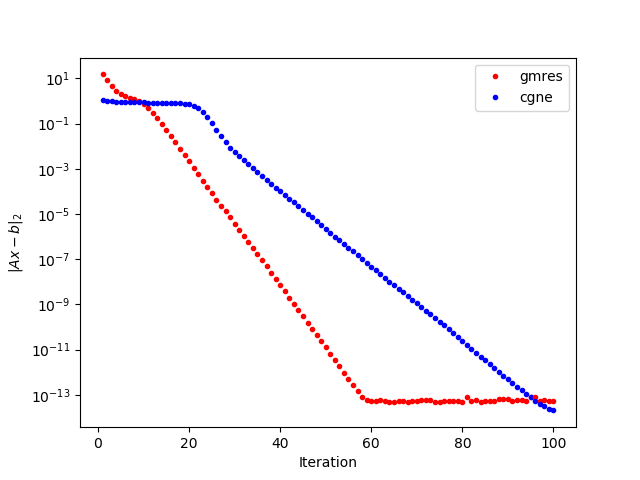
\includegraphics[width=\textwidth]{error_itr.png}
		\caption{Error versus number of iterations required for gmres and cgn for the given system.}
	\end{subfigure}~
	\begin{subfigure}[t]{0.49\textwidth}
		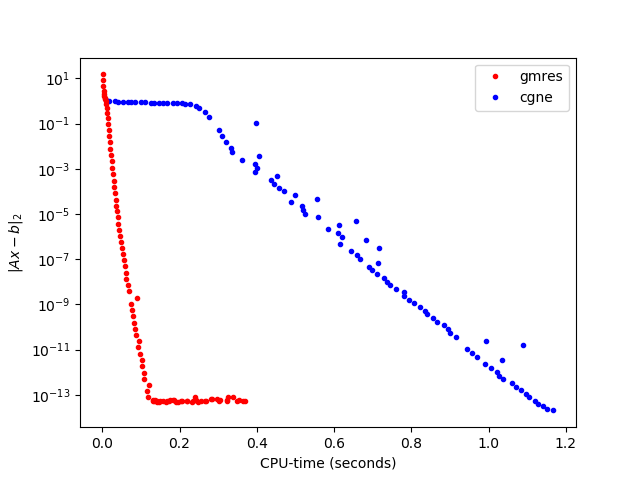
\includegraphics[width=\textwidth]{error_time.png}	
		\caption{Error versus CPU-time required for gmres and cgn for the given system.}
	\end{subfigure}
	\caption{}
	\label{task6}
\end{figure}
The iterates of CGN span a different Krylov subspace than gmres and it is mentioned in the lecture notes on this topic that in most cases, this subspace has worse approximation properties than the usual Krylov subspace used for the gmres iterates. This correspond with what can be observed in Figure \ref{task6}a. 
\subsection{(b)}
The result can be related to the convergence theory for CGN and GMRES. Investigating the eigenvalues of the matrix $B$, it is clear that all eigenvalues are contained in a disk, but for one isolated eigenvalue. However, trying to apply the convergence theory with two discs from the lecture notes is not possible in this case, as the obtained convergence factor is larger than 1. Therefore, one large disc is used and we apply Corollary 2.1.5, choosing $r = 28$ and $c =30 $. The resulting disc and bound is found in Figure \ref{task6b}. Note that for both methods, the bound for the convergence factor is heavily overestimated. 

For CGN, we use the condition number bound for the error in iteration $m$, 
\begin{equation}
\frac{\|e_m\|_2}{\|e_0\|_2}\leq 2\left(\frac{\sqrt{K(B^TB)}-1}{\sqrt{K(B^TB)}+1}\right)^m
\end{equation}
\begin{figure}[h!]
	\centering
	\begin{subfigure}[t]{0.49\textwidth}
		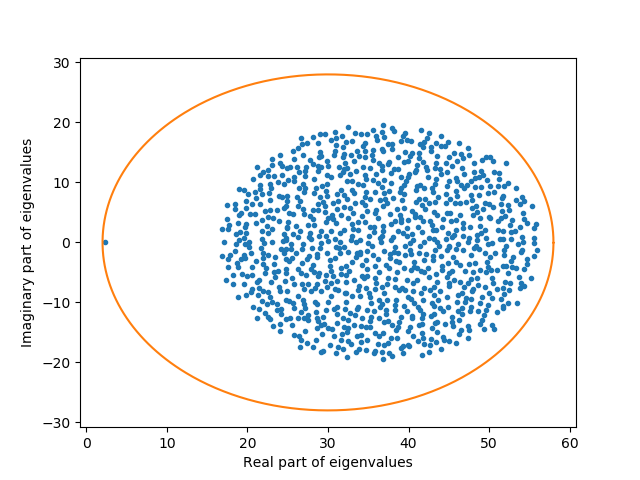
\includegraphics[width=\textwidth]{Eigens.png}
		\caption{Eigenvalues of the matrix B visualised together with disc of convergence used for gmres convergence estimate.}
	\end{subfigure}~
	\begin{subfigure}[t]{0.49\textwidth}
		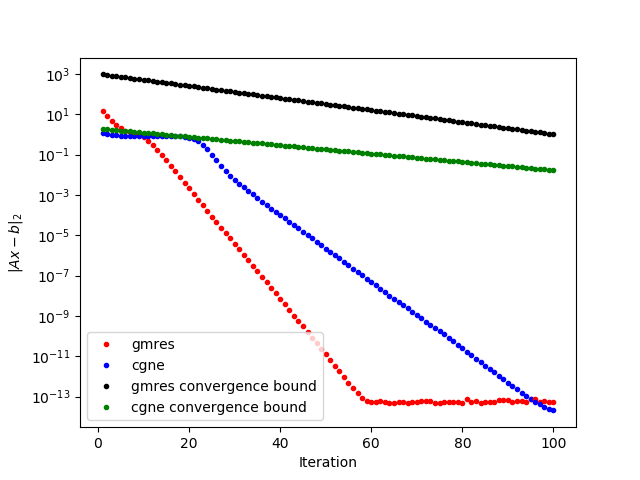
\includegraphics[width=\textwidth]{error_bound.png}	
		\caption{Convergence for gmres and CGN along with estimates of their convergence factors.}
	\end{subfigure}
	\caption{}
	\label{task6b}
\end{figure} 
